\let\negmedspace\undefined
\let\negthickspace\undefined
\documentclass[journal]{IEEEtran}
\usepackage[a5paper, margin=10mm, onecolumn]{geometry}
%\usepackage{lmodern} % Ensure lmodern is loaded for pdflatex
\usepackage{tfrupee} % Include tfrupee package

\setlength{\headheight}{1cm} % Set the height of the header box
\setlength{\headsep}{0mm}     % Set the distance between the header box and the top of the text

\usepackage{gvv-book}
\usepackage{gvv}
\usepackage{cite}
\usepackage{amsmath,amssymb,amsfonts,amsthm}
\usepackage{algorithmic}
\usepackage{graphicx}
\usepackage{textcomp}
\usepackage{xcolor}
\usepackage{txfonts}
\usepackage{listings}
\usepackage{enumitem}
\usepackage{mathtools}
\usepackage{gensymb}
\usepackage{comment}
\usepackage[breaklinks=true]{hyperref}
\usepackage{tkz-euclide} 
\usepackage{listings}
% \usepackage{gvv}                                        
\def\inputGnumericTable{}                                 
\usepackage[latin1]{inputenc}                                
\usepackage{color}                                            
\usepackage{array}                                            
\usepackage{longtable}                                       
\usepackage{calc}                                             
\usepackage{multirow}                                         
\usepackage{hhline}                                           
\usepackage{ifthen}                                           
\usepackage{lscape}
\begin{document}

\bibliographystyle{IEEEtran}
\vspace{3cm}

\title{NCERT 9.4.7}
\author{EE24BTECH11036 - Krishna Patil}
% \maketitle
% \newpage
% \bigskip
{\let\newpage\relax\maketitle}

\renewcommand{\thefigure}{\theenumi}
\renewcommand{\thetable}{\theenumi}
\setlength{\intextsep}{10pt} % Space between text and floats

\textbf{Question} Solve the differential equation:

\begin{center}
$ y \ln(y) \, dx - x \, dy = 0 $
\end{center}

with initial conditions $ x = 1 $ and $ y = e $. \\
\solution \\
\textbf{Step 1: Rearranging the Equation} \\
First, we rewrite the equation in a more convenient form:
\begin{center}
$ y \ln(y) \, dx = x \, dy $
\end{center}

Next, we divide both sides by $ x \ln(y) $:

\begin{center}
$ \frac{dy}{dx} = \frac{y \ln(y)}{x} $
\end{center}

\textbf{Step 2: Separation of Variables} \\
Now, we separate the variables to prepare for integration:

\begin{center}
$ \frac{dy}{y \ln(y)} = \frac{dx}{x} $
\end{center}

\textbf{Step 3: Integration} \\
We now integrate both sides.
\begin{center}
$ u = \ln(y) \implies du = \frac{1}{y} \, dy $ \\
$ \int \frac{1}{u} \, du = \int \frac{1}{x} \, dx $
\end{center}

This leads to:

\begin{center}
$ \ln|u| = \ln|x| + C $
\end{center}

Substituting $ u = \ln(y) $, we have:

\begin{center}
$ \ln|\ln(y)| = \ln|x| + C $
\end{center}

Exponentiating both sides:

\begin{center}
$ |\ln(y)| = C' |x| $
\end{center}

where $ C' = e^C $. Now solving for $ y $, we get:

\begin{center}
$ \ln(y) = C' x $
\end{center}

Exponentiating again:

\begin{center}
$ y = e^{C' x} $
\end{center}

\textbf{Step 4: Applying the Initial Conditions}
To determine the constant $ C' $, we apply the initial condition $ x = 1 $ and $ y = e $:

\begin{center}
$ e = e^{C' \cdot 1} $
\end{center}

Thus, $ C' = 1 $, and the solution to the differential equation is:

\begin{center}
$ y = e^x $
\end{center}


The solution for the differantial equation can be graphically solved using coding by using below logic :

\begin{center} 
$x_0 = 1 $ \\
$y_0 = e $ \\
$ h=0.1 $ \\
$y_{n+1} = y_{n} + h\cdot\brak{\frac{y_{n}\ln{y_{n}}}{x_{n}}}$ \\
$x_{n+1} = x_{n} + h$ \\
\end{center}

Below is verification \ref{fig:example} :
\begin{figure}[h]  % The 'h' means 'here' (positioning)
    \centering  % Centers the figure
    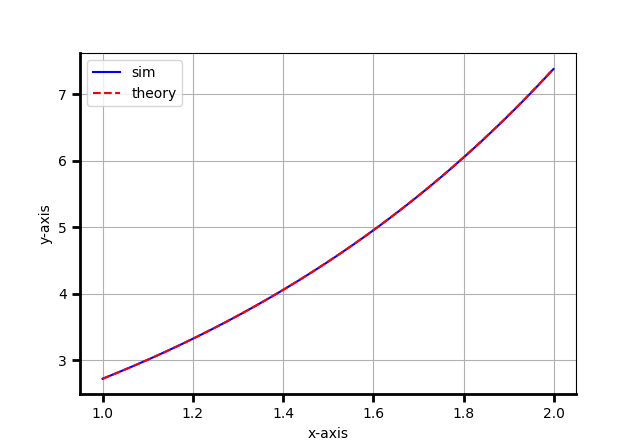
\includegraphics[width=0.5\textwidth]{fig/Figure_1.png}  % Adjust width to 50% of the text width
      \label{fig:example}  % Label for referencing
\end{figure}


\end{document}
